The European Rail Traffic Management System (ERTMS) consists of
several sub-systems. With regards to control and safety, these systems
are typically designed to ensure safe operation of a particular area
of railway known as a scheme plan. Here, we consider open scheme plans
only, i.e., the scheme plans have entry and exit tracks where trains
appear or dissappear, respectively. The ERTMS standard includes
mechanisms of trains can pass between such regions (so-called handover
protocols). In the following, we concentrate on safety within one
region, and leave the handover mechanism for future work.

Figure~\ref{fig:schemeplan} depicts the \emph{scheme plan} for a
junction, which comprises of a track plan, a control table, and
release tables. The \emph{track plan} provides the topological
information of the junction. It consists of X tracks ( e.g.,\ the
track XX), X marker boards (XXX), and a point (P101). The {\em control
table} describes conditions on the setting of \emph{routes}. A
topological route is a piece of railway on which a train can travel
(typically) between two marker boards. For each route, there is one
row in the control table describing the condition under which the
route can be set for use by a train. For example, a train can only
proceed on route X when point P101 is in normal (straight) position
and tracks X, Y, Z are clear. Finally, release tables are sometimes
used to implement sequential release~\cite{} for improving utilisation
of routes, however we will not consider this feature within this work.

Assumptions in the scheme plan:
\begin{itemize}
\item unidirectional track plans only.
\item Marker Boards always at the end of a track segment.
\item 
Geographic layout: EOA and Marker Board and ``joing of two track
segments'' are the same geographic point.
\item lengths:
50m for a point;
200m for an overlap;
1500m for a normal track.
\item
 speeds: 70mph (sideline) and 120mph (main line); 40mph for crossing a point in reverse direction (?)

\item 
at the begin of each route there is a balise, which trains can use for positioning (ask Siemens)

\item (look carefully at the RBC table -- here we worked out an abstraction)
unclear: how does the RBC figure out: what is the next route for a
train?  Example: there is a train on AC, and route R2 is
available. Then the RBC better does not give a EOA of 1750, as the p02
would be in the wrong position. Just by distance between the balises
and the train it can't be decided if a train is on AC or on BC. 

Naturally, the RBC could store internally, which route has been given to a train. 

However, this would be ``our'' solution - the question is what is the solution at Siemens.


\item
We deal with open topologies, where there are designated entry and
exit tracks. We always assume that entry tracks have -- at thier end
-- a marker board.

In order to aviod collisions on the first overlap after
an entry track, we require that trains can only enter an entry track,
if the first overlap is free.

In our example: AA must be free for a train to enter on the entry track.

\item 
The RBC is ``passsive'' rather than pro-active. The RBC makes a ``proceed request'' only after a train has requested a MA. In ERTMS this is not necessarily the case.

\item
Trains request a new MA the moment they start to break. In ERTMS, there are various stragies possible.

\end{itemize}

\begin{figure}
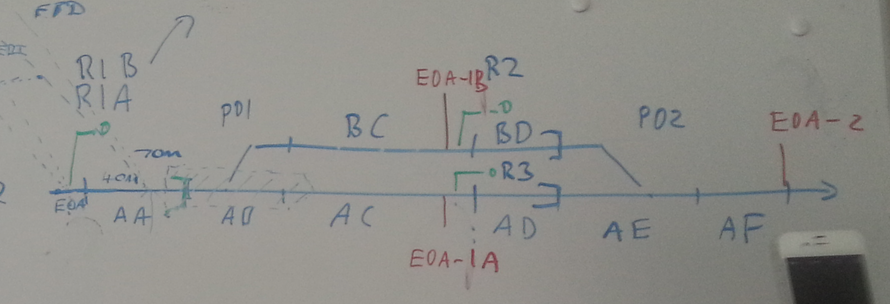
\includegraphics[width=\linewidth]{trackplan.png}
\caption{The scheme plan for a typical junction.}
\label{fig:schemeplan}
\end{figure}

\begin{verbatim}
Control table: 
Route Normal Reverse Clear 
R1A     P01          AA,AB,AC,AD 
R1B            P01   AA,AB,BC,BD 
R2             P02   BD, AE, AF 
R3      P02          AD,AE,AF

Release Tables:
P01: R1A - AC
     R1B - BC
P02: R2 - AF
     R3 - AF

RBC - Table
Route begin end   possible continuation routes
R1A   0     1750  R3
R1B   0     1750  R2
R2    1750  3500  - 
R3    1750  3500  -
\end{verbatim}


\begin{verbatim}

Communication between Components:
=======================
Interlocking (instant behaviour, all are equations)
=============================
Attributes of an interlocking:
RoutesSet Map {NamedRoutes->Bool}
\alert{PointsLocked Map {Points -> Bool}[was RoutesLocked]
PointsNormal Map {Point -> Bool}
PointsReverse Map {Point -> Bool}
TrackOccupation {Track -> Bool}
\end{verbatim}

\begin{verbatim}

Message from controller (message: routename to be set).
Case 1: route already set.
        do nothing (i.e. message is deleted.)
        Alternatives 1: it could doublecheck occupany and point settings.
        Alternative 2: we could set it again. 

Case 2: route not set and \alert{points are locking in conflicting 
                          position or clearpart of route not free}
        do nothing.

Case 3: route not set, check whether all segments in clear table are free and 
            \alert{points are set correct or free to move, i.e. not locked (in conflicting pos.)}
        do: - set route (update map), set points for this route (update map)
            - message to RBC (send RouteSet map).
          

Message from Train: (message contains new occupied tracksegment)
        do: - sets trackseg to be occupied, free up previous one.
            - release: 
              if new tracksegment is mentioned in releasetable (part of control table)
              remove \alert{Point from PointsLocked}
            - sends TrackOccupation map to RBC.
               
        Note there is a separate rule when trains leaves exit tracksegement
        (message countains topological route).

         
          
Message from RBC: (contains routename = request to proceed on a route)
Case 1: route is still set:
        do: - \alert{lock points on route.}
            - sent proceed message to RBC.
 
Case 2: route not set anymore.
             - do nothing.


Question: how does train know where to go next?
Currently in Andi's module next depends on currentsegment and route. 
[This might need to change to  current point setting from interlocking. 
We will do this when looking at scenarios.]


RBC:
====
SetRouteNames (subset of RouteNames)
ProceedPossible (subset of SetRouteNames) 

instead of :TrainRoutemap: Map {Train -> Route}
designatedRoutes (set of Pairs of TrainId and RouteNames) 
[Note both directions should be available TrainId-> RouteName, RouteName->TrainId]



Message from train (contains movement authority request:
                    current track (!) + train id.)
     do: computes current route from TrainRouteMap
         checks whether there is in RoutesSet a suitable follow up one

         Case 1: there is no suitable one, delete MA request.
         Case 2: there a suitable follow-up route in SetRoutes,
               
                 sends message request-to-procceed(routename) to IX  (Id needed?)
 
       
Message from interlocking: proceed(routename)
          RBC puts Routename into ProceedPossible      

          For every RN in ProceedPossibe:
               - compute eoA(RN)
               - compute train form designated Id-Routename
               - send MA(RN) to train
               - remove RN from ProceedPossible.

               
     

            


Controller:
==========
Sends Message: Routerequest (random route), every 10 time steps (can be made random)




\end{verbatim}



Once such a scheme plan has been designed, a number of control systems
are implemented based around it. Figure~\ref{fig:arch} presents an
overview of these systems and the information flow between
them~\footnote{Here some details may differ between individual rail
providers. We present an overview of the systems used by Siemens Rail
UK.}. The modelling and verification of these systems forms the main
focus of this work.

\begin{figure}[h]
\includegraphics[width=\linewidth]{Images/architecture.png}
\caption{ERTMS control architecture}
\label{fig:arch}
\end{figure}

The controller (manual or computerised) is responsible for controlling
the flow of trains through the railway network. The controller
completes this task by sending route requests to the
interlocking. These route requests are dependent upon elements such as
the current timetable to be adhered to and details on congestion
within the network.

The interlocking is responsible for the setting and granting of
requested routes.  Once the controller has requested a route, the
interlocking will use information on current track occupation and
point settings (from the track equipment) to determine if it is safe
for the requested route to be set. The process for determining whether
or not a route can be set is based around the conditions stipulated by
the control table, see Figure~\ref{fig:schemeplan}. Once the
interlocking has checked that all points on the route are free to move
or set in the right direction, it will send a route available message
to the RBC. This informs the RBC that the route is free for use,
however not reserved for a train. The process of locking a route for a
particular train is only initiated when the RBC sends a request to
proceed message informing the interlocking that there is a train that
would like to use an available route. On receiving this message, the
interlocking will then ensure that, based on the control table, all
tracks for the route are free and that the points are indeed locked in
the required positions. Once this step is completed, the interlocking
sends a proceed message to the RBC indicating that a train can use the
route.

The RBC's main responsibility is to take the route information
presented by the interlocking and use it to manage the movement of
trains across geographic positions on the railway. To do this, the RBC
and trains use the notion of a \emph{movement authority}. A movement
authority is an area of geographical railway that a train is permitted
to move within. The furthest point along the railway to which a train
is permitted to move is indicated by a point known as the \emph{end of
authority} (EoA)which is given to a train by the RBC. As a train moves
across the railway network, it uses beacons on the track to
continually calculate its position. When it is nearing its EoA, it
makes a new movement authority request to the RBC indicating that it
would like its movement authority to be extended. After receiving this
request, the RBC will map the physical location of the train to an
available continuation route that has been presented to it by the
interlocking~\footnote{At this point, there should be maximally one
route available that matches a particular train. This is ensured by
the requests from the controller and also the ability of the
interlocking to deny requests for conflicting routes}. It will then
issue the request to proceed message to the interlocking for this
route. Once the RBC has received a proceed message from the
interlocking, it will compute based on the route that has been granted
a new EoA for the train. This new EoA is then sent to the train.

In this setting, we consider several safety properties:
\emph{collision-freedom} excludes two trains occupying the same track ... 


\begin{verbatim}
The hope would be that - with the described mistakes in the static, location dependent data - the Maude search command can find these violations

Search might be faster, as the model checking is implemented on top of Maude - while search is a function implemented within Maude.

Basic assumption: the models of the dynamic behaviour of train, rbc, interlocking are correct - the mistakes we are looking for are within the parameters to these models.

---------

These are three classical safety properties, inherited from solid
state interlockings. However, here we write them down in the language
of Movement Authorities:

collision freedom:
no overlapping Movement-Authorities &
for all trains t: t stays within its Movemen-Authority

run-through freedom:
for all MA: Movement-Authority, forall points p:
  p is within MA => p is in the "right" position

 ->   -----\
            \
 ->   ------------------------ A

            p

 if a train comes on the upper line, and its movement authority ends
 at A, then p is in reverse and not in normal.


no moving point under train (derailment freedom):
for all MA: Movement-Authority, forall points p:
 p is within MA => p is not moved.

Interlockings:
--------------

Mistakes in the control and in the relase table can lead to violation of all three of
the above different safety properties.

How to produce violations of these:

Scenario 1 (collision): in the control-table, a track is missing in the clear part
of a route name; can lead to a collision.

Scenario 2 (collision): in the control-table, for the row belonging to a route
name, a point is put in reverse rather than normal or vice versa;
can lead to a collision (when a second train follows the first one
on the very same route - as the clear part can checks that the wrong
tracks are free).

Scenario 3 (run-through): the track-plan includes a point for joining two routes; in
the control-table, for the row belonging to one of the joining route
names, a point is put in reverse rather than normal or vice
versa. This can lead to a run-through.

Scenario 4 (moving point): in the release table, the lock of a point
is released too early for a route name. This might lead to moving a
point under a train.

[hint: locks and release tables are probably not part of our model]

Trains:
-------

Scenario 5 (collision): A train has a physical braking behaviour (used
to determine the speed). The train driver enters a braking rate (used
to compute the breaking point). If the entered braking rate is
"faster" than the physical breaking rate, then the train won't stay
within its movement authority. In this case, we can't guarantee
collision freedom (as defined above) anymore. This will require two
different constants in the Maude model of a train.

[A possible extension of the model might be to add an ATP automaton,
which takes over in case the train fails to stop at the end of
Movement Authority. The ATP should then stop the train on the
overlap. Thus, we would not have a collision.]

RBC:
----

static data / location dependent (as parameters of the RBC):
- clear part of the control table
- map: position on the track * P(Route-Names) -> Movement Authorities

dynamic data: set of currently set Route-Names

Questions to Siemens:

- Can it happen that the control table in the Interlockint and the
control table (part) in the RBC differ?

- Is the idea of the above map in the RBC a realistic one?

Unclear: what are the effects if there are mistakes in the static,
location dependent data of the RBC?

Scenario 6 (collision): In the map, the movement authority given out
is too long. Then, even if the train stay within its movement
authority, a collision could happen.

Scenario 7 (??): In the clear part of a control table, a track is
missing. We are not sure about the effect.
\end{verbatim}

